%!TEX TS-program = xelatex

\documentclass[t]{beamer}

\usetheme{Hannover}
\usecolortheme{rose}

%%% Работа с русским языком
\usepackage[english,russian]{babel}   %% загружает пакет многоязыковой вёрстки
\usepackage{fontspec,xltxtra,xunicode}      %% подготавливает загрузку шрифтов Open Type, True Type и др.
%\defaultfontfeatures{Ligatures={TeX},Renderer=Basic}  %% свойства шрифтов по умолчанию
\setmainfont[Ligatures={TeX,Historic},
SmallCapsFont={Brill},
SmallCapsFeatures={Letters=SmallCaps}]{Brill} %% задаёт основной шрифт документа
\setsansfont{Brill}                    %% задаёт шрифт без засечек
\setmonofont[Ligatures=NoCommon]{DejaVu Sans}
\newfontfamily\SYM{Brill}
\usepackage{indentfirst}
%%% Дополнительная работа с математикой
\usepackage{amsmath,amsfonts,amssymb,amsthm,mathtools} % AMS
\usepackage{icomma} % "Умная" запятая: $0,2$ --- число, $0, 2$ --- перечисление

%%% Работа с картинками
\usepackage{wrapfig} % Обтекание рисунков текстом
\usepackage{rotating}
\usepackage{fixltx2e}
\usepackage{hhline}
\usepackage{lscape}

%%% Работа с таблицами
\usepackage{array,tabularx,tabulary,booktabs} % Дополнительная работа с таблицами
\usepackage{longtable}  % Длинные таблицы
\usepackage{multirow} % Слияние строк в таблице

\usepackage{multicol} % Несколько колонок

%%% Страница
%\usepackage{fancyhdr} % Колонтитулы
% 	\pagestyle{fancy}
 	%\renewcommand{\headrulewidth}{0pt}  % Толщина линейки, отчеркивающей верхний колонтитул
% 	\lfoot{Нижний левый}
% 	\rfoot{Нижний правый}
% 	\rhead{Верхний правый}
% 	\chead{Верхний в центре}
% 	\lhead{Верхний левый}
%	\cfoot{Нижний в центре} % По умолчанию здесь номер страницы

\usepackage{setspace} % Интерлиньяж
%\onehalfspacing % Интерлиньяж 1.5
%\doublespacing % Интерлиньяж 2
\singlespacing % Интерлиньяж 1

\usepackage{subfig} % подкартинки
\usepackage{lastpage} % Узнать, сколько всего страниц в документе.
\usepackage{soul} % Модификаторы начертания
\usepackage{bbding}
\usepackage{hyperref}
\usepackage{tikz} % Работа с графикой
\usepackage{pgfplots}
\usepackage{pgfplotstable}
\usepackage{verbatim}

\usepackage{attachfile2}
 \attachfilesetup{appearance=true,
color=0 0 0
 }
\usepackage{alltt}

%%% Лингвистические пакеты
%\usepackage{savetrees} % пакет, который экономит место
\usepackage{forest} % для рисования деревьев
\usepackage{vowel} % для рисования трапеций гласных
\usepackage{natbib}
\bibpunct[: ]{[}{]}{;}{a}{}{,}
\usepackage[nogroupskip,nopostdot, nonumberlist]{glossaries}
%\usepackage{glossary-mcols} 
%\setglossarystyle{mcolindex}
\usepackage{philex} % пакет для примеров
\newcommand{\mytem}{\item[$\circ$]}
\addto\captionsrussian{
\renewcommand{\refname}{}}

\newcommand{\apostrophe}{\XeTeXglyph\XeTeXcharglyph"0027\relax}
\usetikzlibrary{patterns}

\usepackage{ulem}
\usepackage{subfig}
\setbeamercolor{alerted text}{fg=red!13!blue}
\setbeamersize{text margin left=4mm,text margin right=1mm} 
\setbeamertemplate{navigation symbols}{
	\usebeamerfont{footline}%
    \usebeamercolor[fg]{footline}%
    \hspace{1em}%
    {{\small презентация доступна: \href{http://goo.gl/F6pC3o}{\textbf{http://goo.gl/F6pC3o}}}
    \hspace{4.3cm}
    \insertframenumber/\inserttotalframenumber\vspace{0.5mm}}}
\newcommand{\mcrot}[4]{\multicolumn{#1}{#2}{\rlap{\rotatebox{#3}{#4}~}}} 
% начало
\title[]{Матрицы расстояний, кластеризация \\ и деревья решений}
\author[]{Г. Мороз}
\date{}
\begin{document}
\frame{\titlepage}
\section{метрики расстояний}
\subsection{метрики расстояний}
\begin{frame}{Матрицы расстояний}
\textbf{Матрица расстояний} — это матрица $n\times n$, которая содержит значения меры расстояния/сходства между объектами в метрическом пространстве. Существует уйма мер расстояния/сходства, выбор из которых зависит от типа данных. К сожалению, \textbf{не} существует универсального алгоритма выбора метода, так что это остается на откуп исследователям. Кроме того, схожие методы, зародившиеся в биологии, называют string metric: они определяют расстояния между строками (расстояние Хэмминга, расстояние Левинштейна и т. п.)
\end{frame}
\begin{frame}{Бинарные данные: коэффициент Жаккара}
Компаративисты сравнивают языки на основе количества общих когнатов в списке Сводеша. Таким образом, для стословника составляются бинарные матрицы, которые отражают, какой когнат в каком идиоме встретился.
\scriptsize
\begin{alltt}
\begin{tabular}{lll}
df <- data.frame(& Lithuanian = & c(1, 1, 1, 1, 0), \\ 
 & Latvian = & c(1, 1, 1, 0, 0), \\ 
 & Prussian = & c(1, 1, 0, 0, 0), \\ 
 & ChurchSlavonic = & c(0, 0, 0, 0, 1)) \\ 
\end{tabular}
\end{alltt}
\normalsize
Для каждой пары идиомов строим таблицу сопряженности:\\
\hfill
\scriptsize
\begin{tabular}{|c|c|c|c|}
\hline
 \multicolumn{ 2}{|c|}{}  & \multicolumn{ 2}{c|}{идиом i} \\ \cline{ 3- 4}
 \multicolumn{ 2}{|c|}{}  & 1 & 0 \\ \hline
\multirow{2}{*}{идиом j} & 1 & a & b \\ \cline{ 2- 4}
\multicolumn{ 1}{|c|}{} & 0 & c & d \\ \hline
\end{tabular}
\normalsize
\hfill ~\\
Коэффициент Жаккара расчитывается по формуле:\\
$$s(i, j) = \frac{a}{a+b+c} \hspace{15mm} d(i, j) = \frac{b+c}{a+b+c}$$
В работе \citep{gower86} есть и другие методы (14 шт.). Большинство из них есть в функции \scriptsize\verb"dist.binary()"\normalsize\ пакета \scriptsize\verb"ade4"\normalsize.
\end{frame}
\begin{frame}{Бинарные данные: коэффициент Жаккара}
\scriptsize
\begin{alltt}
\begin{tabular}{lll}
df <- data.frame(& Lithuanian = & c(1, 1, 1, 1, 0), \\ 
 & Latvian = & c(1, 1, 1, 0, 0), \\ 
 & Prussian = & c(1, 1, 0, 0, 0), \\ 
 & ChurchSlavonic = & c(0, 0, 0, 0, 1)) \\ 
\end{tabular}
\\
df <- t(df) \hfill \# кластеризации любят держать признаки в строках\\
dm <- \alert{dist}(df, \alert{method = "binary"})\bigskip\\
dm \hfill \# матрица расстояний\\
\alert{
\begin{tabular}{lrrr}
 & Lithuanian & Latvian & Prussian \\ 
Latvian & 0.2500000 &  &  \\ 
Prussian & 0.5000000 & 0.3333333 &  \\ 
ChurchSlavonic & 1.0000000 & 1.0000000 & 1.0000000 \\ 
\end{tabular}}\\
round(100*(dm)) \hfill \# удобнее смотреть\\
\alert{
\begin{tabular}{lrrr}
 & Lithuanian & Latvian & Prussian \\ 
Latvian & 25&  &  \\ 
Prussian & 50 & 33 &  \\ 
ChurchSlavonic & 100 & 100 & 100\\ 
\end{tabular}}\\
\end{alltt}
\normalsize
\end{frame}
\begin{frame}{Небинарные категории: в бинарные}
На основе WALS.
\scriptsize
\begin{alltt}
df <- data.frame(\\
~~~~order = c("SVO", "SOV", "SVO", "VOS"),\\
~~~~gender = c("3", "0", "0", "0"),\\
~~~~future = c("non.inflect", "inflect", "non.inflect", "non.inflect"),\\
~~~~row.names = c("English", "Turkish", "Estonian", "Malagasy"))\\
df\\
\alert{
\begin{tabular}{lrrr}
 & order & \multicolumn{1}{l}{gender} & future \\ 
English & SVO & 3 & non.infl \\ 
Turkish & SOV & 0 & infl \\ 
Estonian & SVO & 0 & non.infl \\ 
Malagasy & VOS & 0 & non.infl \\ 
\end{tabular}} \medskip\\
\alert{model.matrix( \textasciitilde . -1, data=df)\\
\begin{tabular}{lrrrrr}
 & \multicolumn{1}{l}{orderSOV} & \multicolumn{1}{l}{orderSVO} & \multicolumn{1}{l}{orderVOS} & \multicolumn{1}{l}{gender3} & \multicolumn{1}{l}{futurenon.infl} \\ 
English & 0 & 1 & 0 & 1 & 1 \\ 
Turkish & 1 & 0 & 0 & 0 & 0 \\ 
Estonian & 0 & 1 & 0 & 0 & 1 \\ 
Malagasy & 0 & 0 & 1 & 0 & 1 \\ 
\end{tabular}}
\end{alltt}
\normalsize
\end{frame}
\begin{frame}[fragile]{Числовые категории}
Если категории числовые, то чаще всего используют:
\begin{itemize}
\mytem евклидово расстояние \hfill \scriptsize\verb|method = "euclidean"|\normalsize
\mytem расстояние городских кварталов \hfill \scriptsize\verb|method = "manhattan"|\normalsize
\end{itemize}
\begin{center}
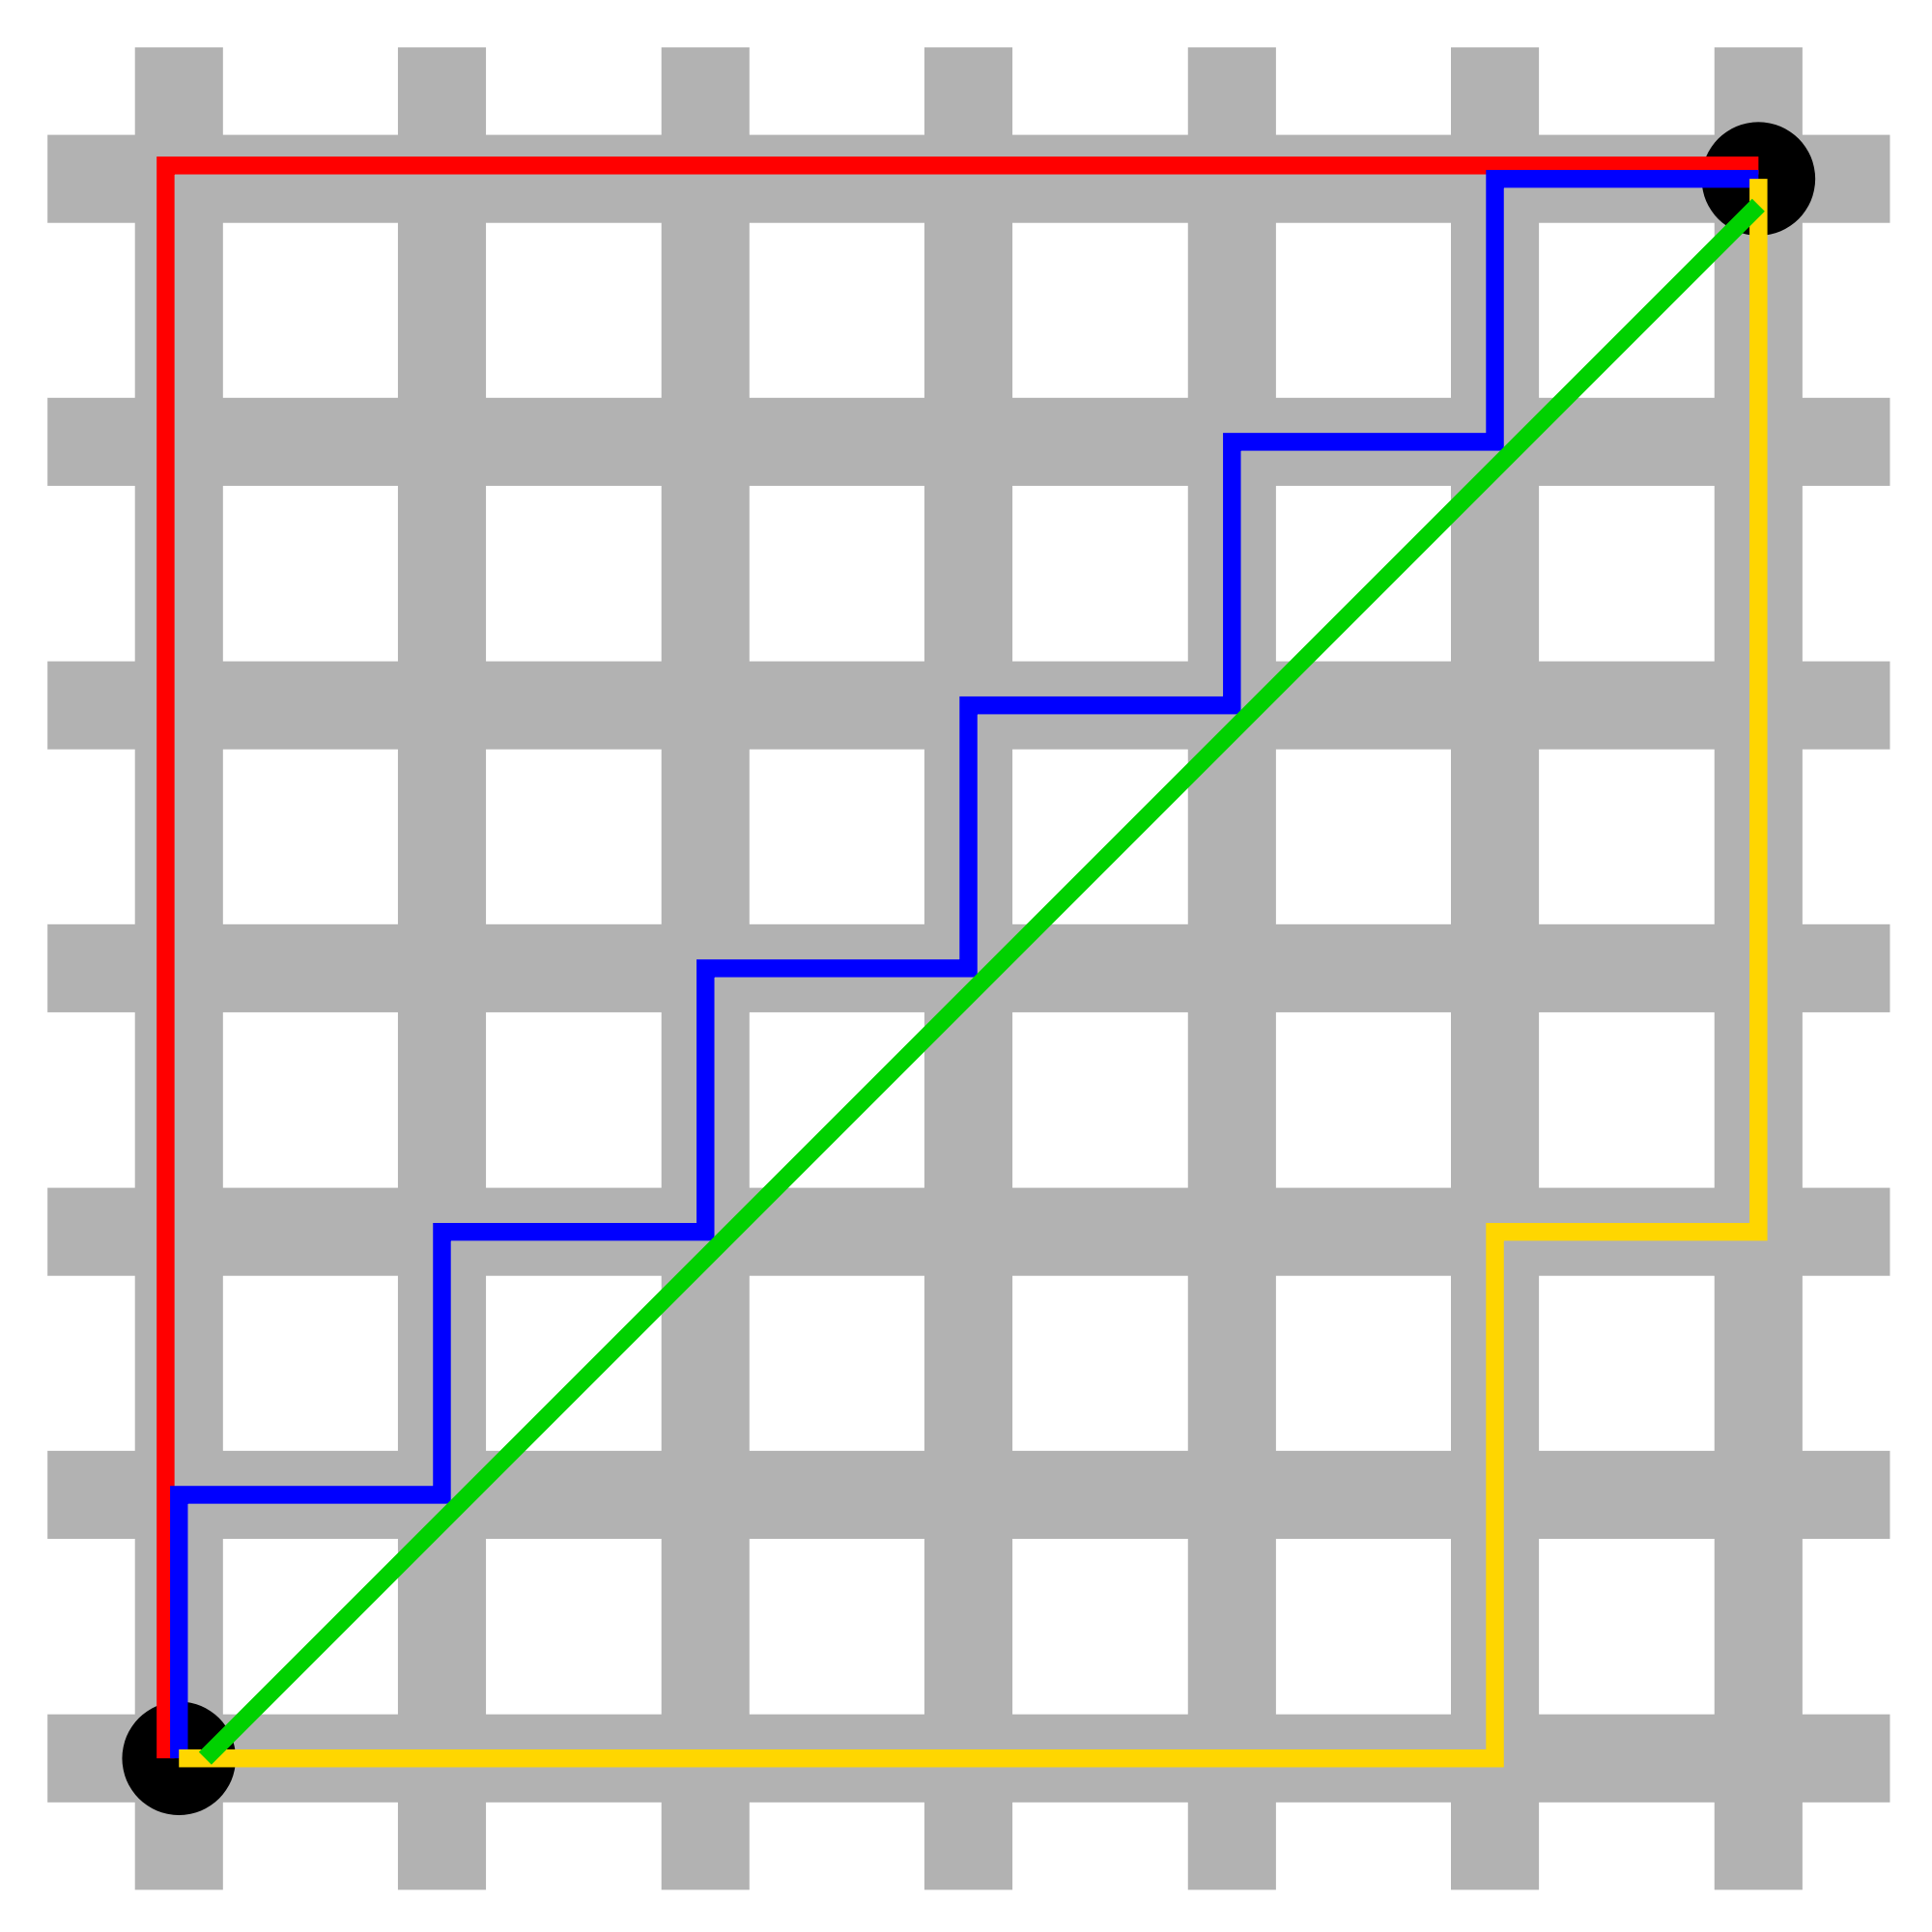
\includegraphics[width=0.4\linewidth]{eucmanhattan.png}
\end{center}
Картинка из \href{https://upload.wikimedia.org/wikipedia/commons/0/08/Manhattan_distance.svg}{\alert{Википедии}}: зеленое — евклидово, остальные — манхэттенское.
\end{frame}
\begin{frame}{Смешанные категории}
Для данных содержащих как числовые, так  и категориальные данные используется алгоритм преложенный в работе \citep{gower71}. В целом, если в данных нет пропущенных значений, эта мера достаточно близка к евклидову расстоянию. В R она реализована функцией \scriptsize\verb"daisy"\normalsize\ пакета 
\scriptsize\verb"cluster"\normalsize. Вот пример на основе данных по количеству согласных и наличию абруптивных (\alert{\href{http://web-corpora.net/~agricolamz/2016HSER/correlation_regressions_ejectives.html}{график}}):\\
\scriptsize
\begin{alltt}
df <- read.csv("http://goo.gl/919qoS", row.names = 1)\\
df <- df[sample(1:27, 5),] \hfill \# выборка из данных\medskip\\
\alert{library(cluster)}\\
dm <- \alert{daisy(}df\alert{)}; dm \hfill \# строит матрицу и вызывает ее \medskip\\
\alert{Dissimilarities : \smallskip\\
\begin{tabular}{lllll}
 & Japanese & Hawaiian & Lakota & Pomo \\ 
Hawaiian & 0.15909091 &  &  &  \\ 
Lakota & 0.84090909 & 1.00000000 &  &  \\ 
Pomo & 0.75000000 & 0.90909091 & 0.09090909 &  \\ 
Turkish & 0.20454545 & 0.36363636 & 0.63636364 & 0.54545455 \\ 
\end{tabular}\smallskip\\
Metric :  mixed ;  Types = I, N \\
Number of objects : 5}
\end{alltt}
\normalsize
\end{frame}
\begin{frame}[fragile]{Метрики расстояний для строк}
Для решения ряда проблем NLP было создано несколько метрик для измерения расстояний между строками. Для подсчета этих метрик в R есть несколько пакетов, я приведу примеры использования \alert{пакета \scriptsize\verb"stringdist"\normalsize}. Наиболее популярные в лингвистике расстояния:
\begin{itemize}
\mytem Хэмминга \hfill \# \scriptsize\verb|methood = "h"|\normalsize~
\mytem Левенштейна (\alert{\href{http://leojiang.com/experiments/levenshtein/}{см. визуализацию}}) \hfill \# \scriptsize\verb|methood = "lv"|\normalsize~
\mytem косинусное \hfill \# \scriptsize\verb|methood = "c"|\normalsize~
\end{itemize}
\scriptsize
\begin{alltt}
library(stringdist)
str1 <- "мама"
str2 <- "папа"
stringdist(str1, str2, method = "h")
\alert{[1] 2}\\
str3 <- "мама"
str4 <- c("папа"{}, "рампа"{}, "лада"{}, "рама")
stringdist(str3, str4, method = "lv")
\alert{[1] 2 2 2 1}
\end{alltt}
\normalsize
\end{frame}
\begin{frame}{Cпособы уменьшения размерностей?}
\begin{itemize}
\mytem регрессионный анализ
\mytem кластеризация
\mytem многомерное шкалирование (multidimensional scaling)
\mytem компонентный анализ (principal component analysis)
\end{itemize}
\end{frame}
\subsection{heatmap}
\begin{frame}{heatmap}
Как обычно, есть несколько способов визуализации:
\begin{itemize}
\mytem в Rbase есть функция \scriptsize\verb"heatmap()"\normalsize, но ее настройка — сплошное мучение
\mytem в \scriptsize\verb"ggplot2"\normalsize\ есть \scriptsize\verb"geom\_tile()"\normalsize
\end{itemize}
Обе функции принимают на вход матрицы, так что результат работы функции \scriptsize\verb"dist()"\normalsize надо трансформировать:
\scriptsize
\begin{alltt}
\begin{tabular}{lll}
df <- data.frame(& Lithuanian = & c(1, 1, 1, 1, 0), \\ 
 & Latvian = & c(1, 1, 1, 0, 0), \\ 
 & Prussian = & c(1, 1, 0, 0, 0), \\ 
 & ChurchSlavonic = & c(0, 0, 0, 0, 1)) \\ 
\end{tabular}
\\
df <- t(df) \hfill \# кластеризации любят держать признаки в строках\\
dm <- \alert{as.matrix(}dist(df, method = "binary")\alert{)}
\end{alltt}
\normalsize 
\end{frame}
\begin{frame}{heatmap: ggplot}
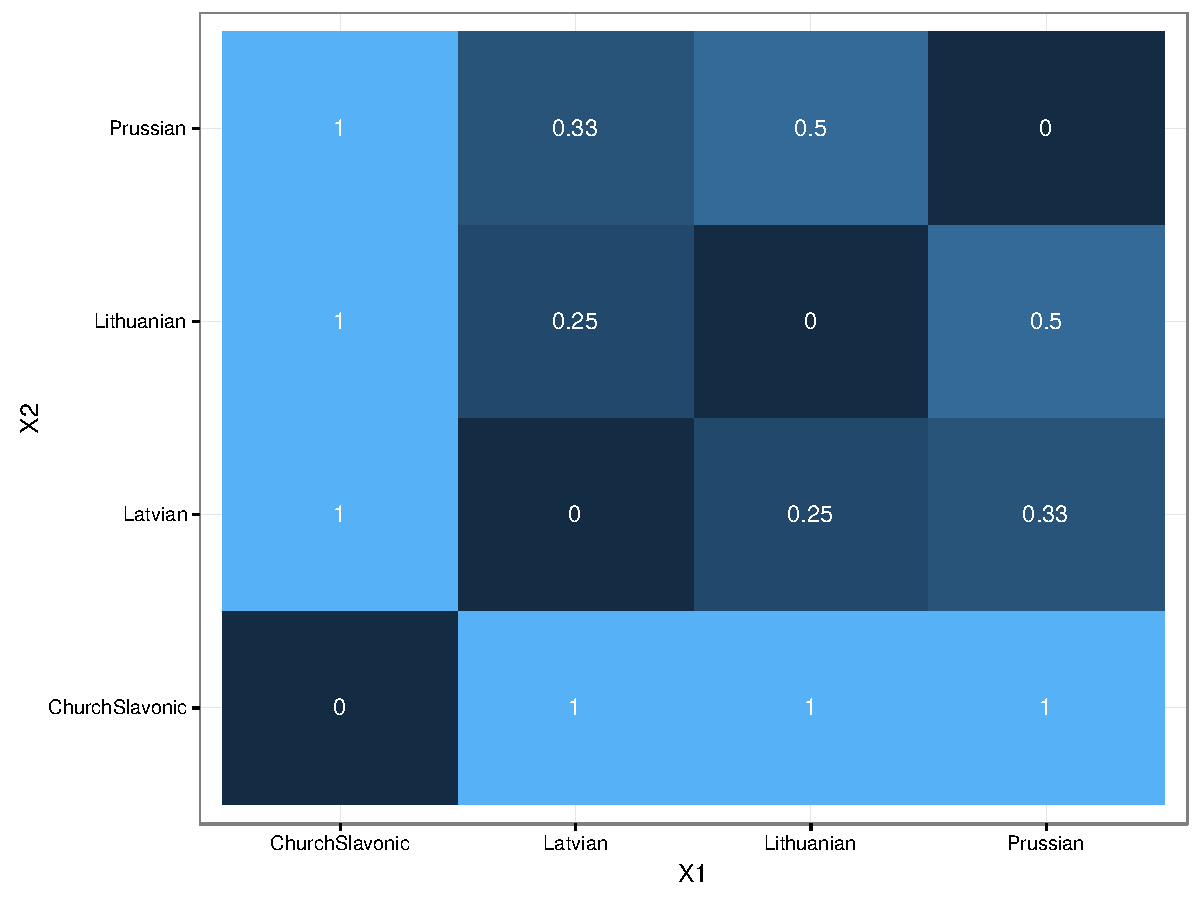
\includegraphics[width=\linewidth]{heatmap.pdf}
\end{frame}
\begin{frame}{heatmap: ggplot}
\scriptsize
\begin{alltt}
\begin{tabular}{lll}
df <- data.frame(& Lithuanian = & c(1, 1, 1, 1, 0), \\ 
 & Latvian = & c(1, 1, 1, 0, 0), \\ 
 & Prussian = & c(1, 1, 0, 0, 0), \\ 
 & ChurchSlavonic = & c(0, 0, 0, 0, 1)) \\ 
\end{tabular}
\\
df <- t(df) \hfill \# кластеризации любят держать признаки в строках\\
dm <- as.matrix(dist(df, method = "binary")) \hfill \# считает расстояния \bigskip\\
library(reshape) \hfill\\
dm.m <- melt(dm) \hfill \# преобразования матрицы для ggplot \bigskip\\

library(ggplot2)\\
ggplot(dm.m, aes(X1, X2, fill=value)) +  \\
~~~~~~~~~~~~\alert{geom\_tile}()+ \hfill \# делает heatmap\\
~~~~~~~~~~~~\alert{geom\_text}(aes(X1, X2, label = \alert{round(}value, 2\alert{)}), \hfill \# пишет значения\\
~~~~~~~~~~~~~~~~~~~~~~~~~~~~~~~color = "white"{}, size = 4)
\end{alltt}
\normalsize
\end{frame}

\section{методы кластеризации}
\begin{frame}{Кластеризация}
Кластеризация — это не метод, а задача, для решение которой придумано множество алгоритмов. Не существует "правильных" методов кластеризации, так как "clustering is in the eye of the beholder" \citep{estivill02}. В презентации рассказывается о представителях двух семейств алгоритмов:
\begin{itemize}
\mytem метод $k$-средних ($k$-means)
\mytem иерархическая кластеризация (hierarchical clustering)
\end{itemize}
\end{frame}
\subsection{k-means}
\begin{frame}{Алгоритм $k$-means}
\vspace{-2.5mm}
Алгоритм $k$-means был разработан в статье \citep{lloyd82}:
\begin{itemize}
\mytem на вход алгоритму подаются данные и $k$ — количество кластеров, на которые эти данные надо поделить;
\mytem произвольно выбираются $k$ точек (центроидов) и рассчитываются ближайшие расстояния (евклидово) от данных точек до центроидов, точки которые ближе всего к некоторому центроиду образуют кластер;
\mytem на основе точек вошедших в кластер строится новый центроид, так чтобы расстояние от всех точек до нового центроида было минимально;
\mytem часть точек становится ближе к новому центроиду и входят в его кластер, а часть от центроида отдаляется и начинают входить в другой/другие кластер/кластеры;
\mytem … все это повторяется, пока на некоторой итерации не происходит изменение положения центроидов.
\end{itemize}
Naftali Harris сделал \alert{\href{http://www.naftaliharris.com/blog/visualizing-k-means-clustering/}{визуализация $k$-means}}.
\end{frame}
\begin{frame}{Задача}
В описании нанайского языка есть гласные i, ɪ и ə (в данных закодированы i, I, e соответственно), однако совсем не понятно, одинаково ли произносят гласные i и ɪ современные носители. В датасет записаны F1 и F2 этих трех гласных, произнесенных в нанайских словах шестью нанайцами из двух селений Найхин и Джуен. Если F1 и F2 достаточно для описания разницы между этими гласными, то тогда они должны кластеризоваться.
\end{frame}
\begin{frame}{Задача}
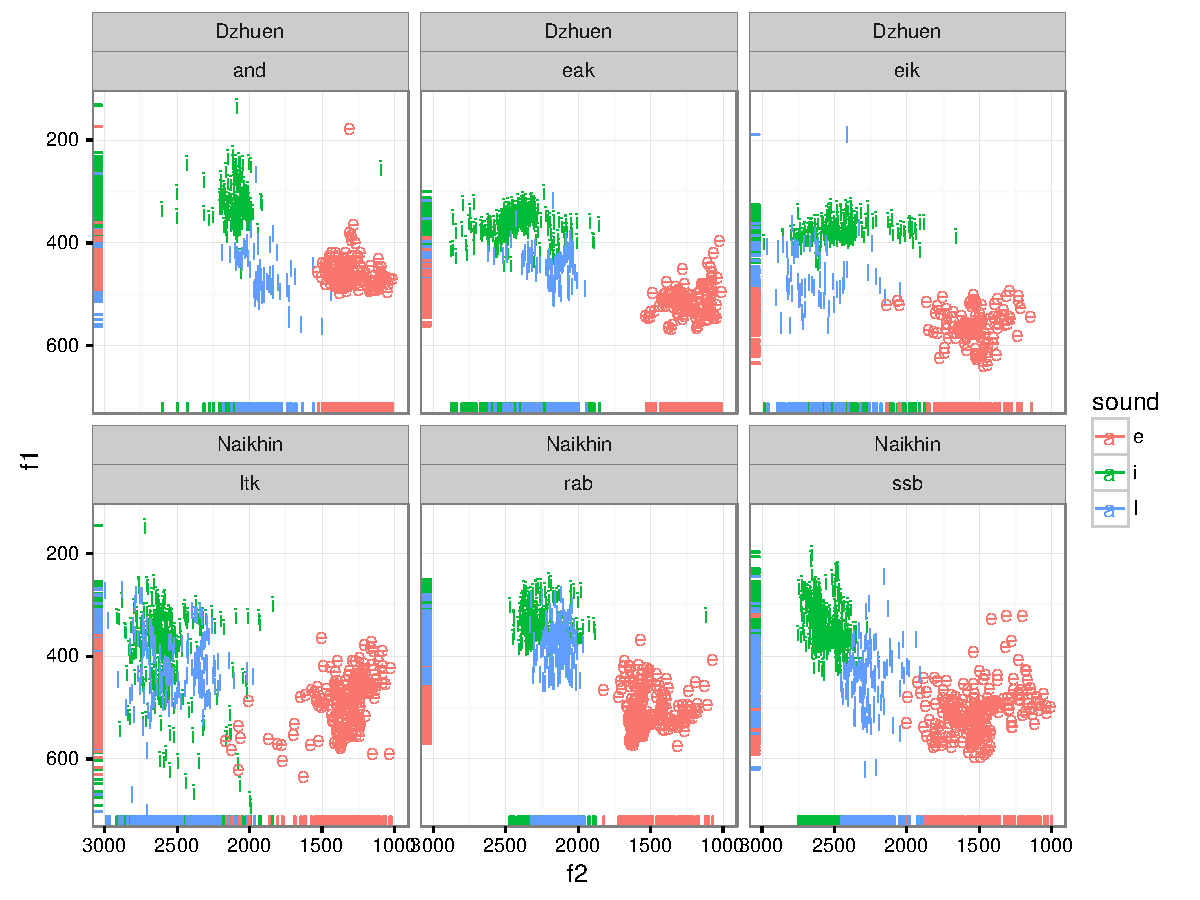
\includegraphics[width=\linewidth]{nanai.pdf}
\end{frame}
\begin{frame}{$k$-means}
Нашим примером будет носитель ssb:
\scriptsize
\begin{alltt}
n <- read.csv("http://goo.gl/YPMyl2"{}, sep = ";")\\
n <- n[n\$dictor == "ssb"{},]\bigskip\\
dm <- dist(n[, c(5,6)])\\
set.seed(5) \hfill \# устанавливаем определенное значение рандомизатора\\
n.cl <- \alert{kmeans}(dm, \alert{centers = 3}) \hfill \# датафрейм, k\\
n.cl\alert{\$cluster} \hfill \# кластер каждой точки\\
n.cl\alert{\$centers} \hfill \# координаты центроидов\\
\end{alltt}
\end{frame}
\begin{frame}{Визуализация $k$-means: R-base}
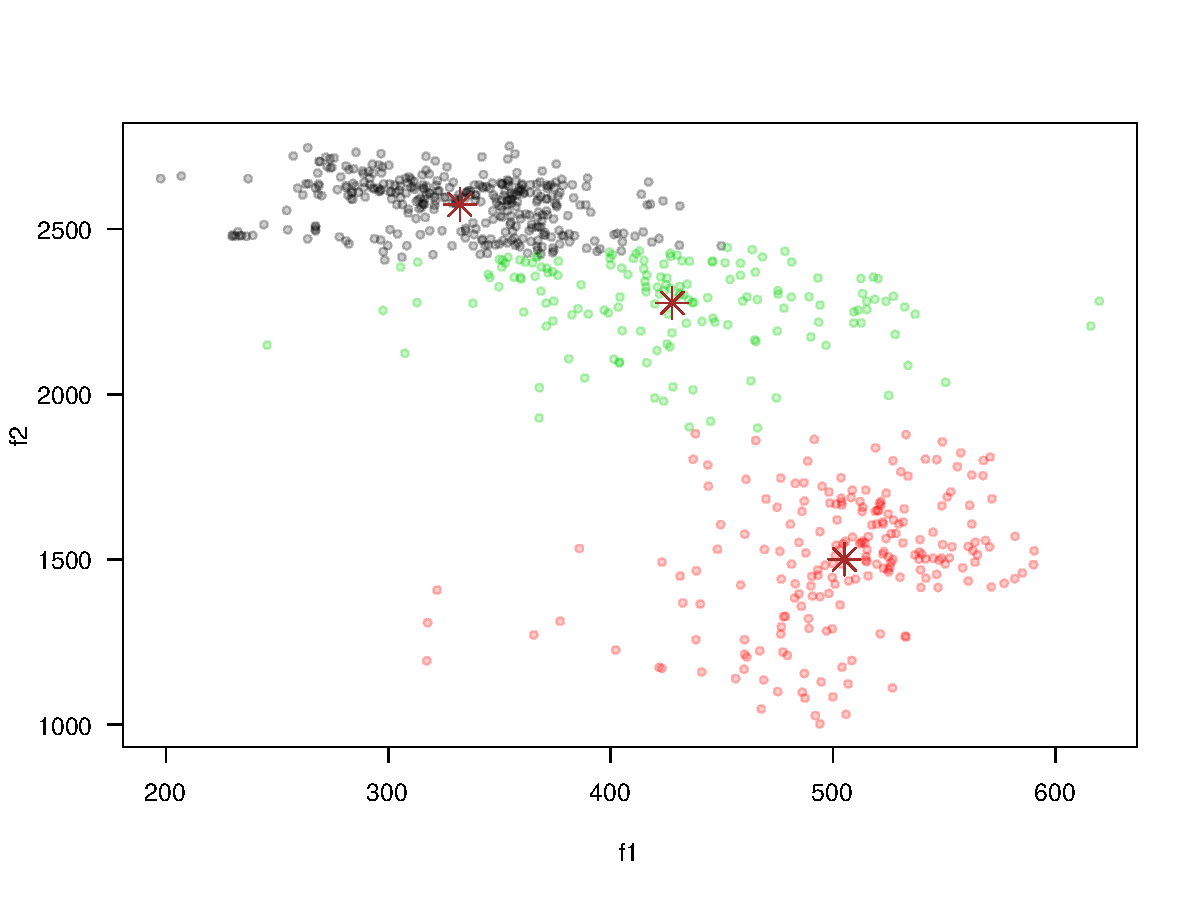
\includegraphics[width=\linewidth]{nanaikmeansrbase.pdf}\\
\scriptsize
\vspace{-3mm}
\begin{alltt}
plot(n[, c(5,6)], \hfill \# данные\\
~~~~~~~~\alert{col = n.cl\$cluster}) \hfill \# раскрашиваем по кластеру\\
points(\alert{n.cl\$centers}, col = "brown"{}, pch = 8, cex = 2) \hfill \# центроиды\\
\end{alltt}
\normalsize
\end{frame}
\begin{frame}{Визуализация $k$-means: ggplot2}
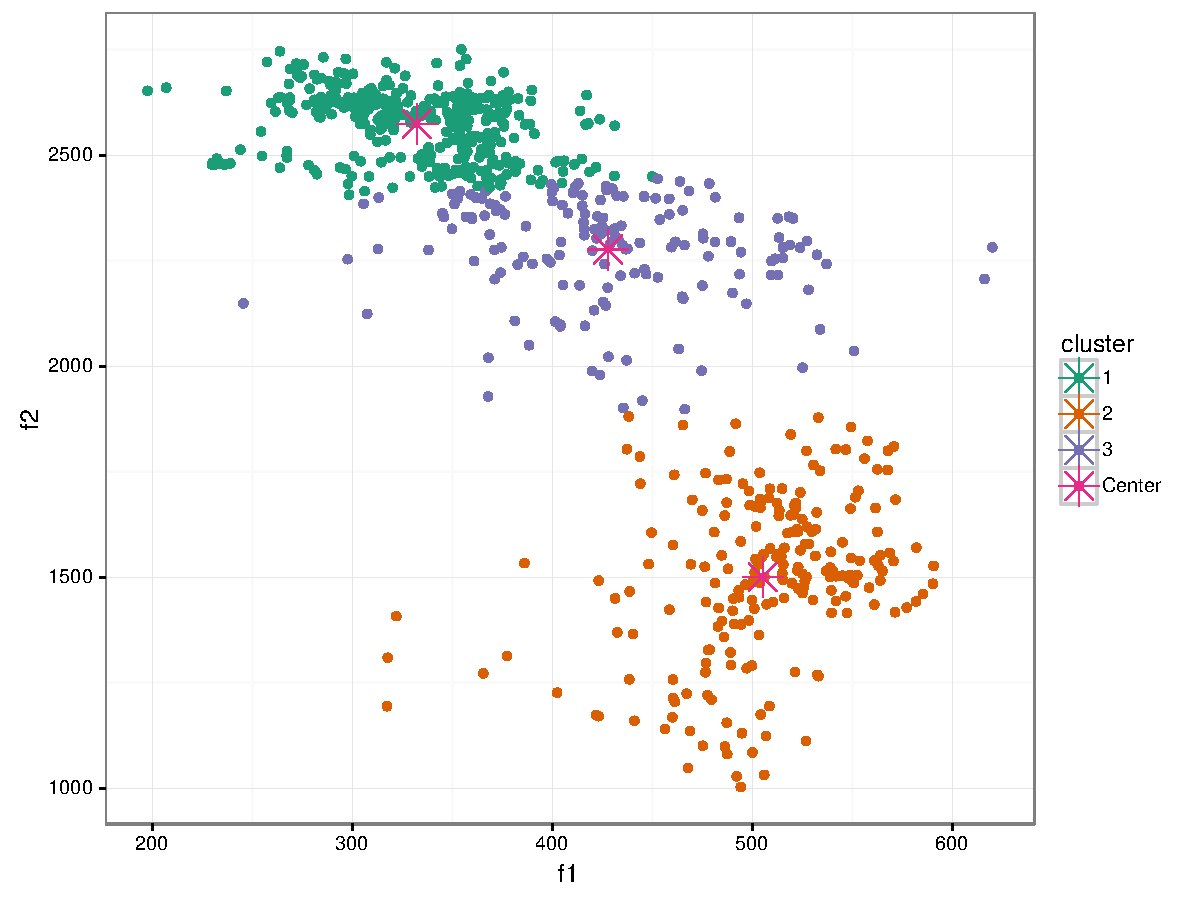
\includegraphics[width=\linewidth]{nanaikmeansggplot.pdf}\\
\end{frame}
\begin{frame}{Визуализация $k$-means: ggplot2}
\scriptsize
\begin{alltt}
n\$cluster <- factor(n.cl\$cluster) \hfill \# добавляет кластеризацию в дф\\
centers <- as.data.frame(n.cl\$centers) \hfill \# создает дф с центроидами \bigskip\\
library(ggplot2)\\
ggplot(\alert{data=n}, aes(x=f1, y=f2, \alert{color=cluster})) + \\
~~~~~geom\_point() + \\
~~~~~geom\_point(\alert{data=centers}, aes(x=f1,y=f2, color='Center'), \\
~~~~~~~~~~~~~~~~~~~~shape = 8, size = 5) \\
\end{alltt}
\normalsize
\end{frame}
\begin{frame}{$k$-means: продолжение}
И что дальше? В наших данных есть информация о произнесениях, так что можно сравнить (следующий слайд) результат работы k-means (обозначено цветом) с тем, что ожидалось в данных словах (обозначено буквой) и посмотреть сколько раз $k$-means ошибся (слайд через один):\\
\vfill
\begin{center}
\small
\begin{tabular}{lccccccc}
 & and & eak & eik & ltk & rab & ssb \\ 
correct & 393 & 426 & 278 & 515 & 549 & 682 \\ 
mistaken & 27 & 61 & 99 & 148 & 102 & 43 \\ 
 &  &  &  &  &  \\ 
 & and & eak & eik & ltk & rab & ssb \\ 
correct & 0.94 & 0.87 & 0.74 & 0.78 & 0.84 & 0.94 \\ 
mistaken & 0.06 & 0.13 & 0.26 & 0.22 & 0.16 & 0.06 \\ 
\end{tabular}
\normalsize
\end{center}
\end{frame}
\begin{frame}{Кластеры $k$-means}
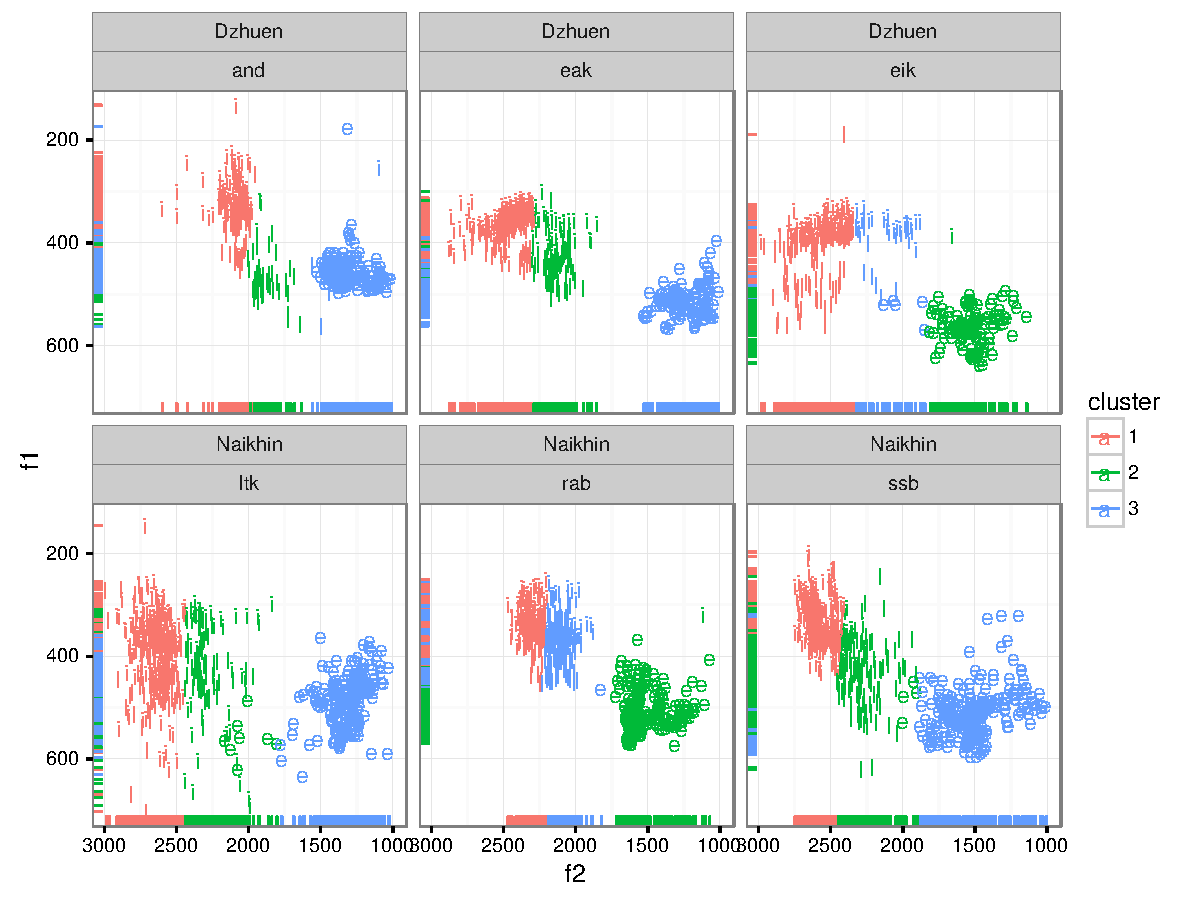
\includegraphics[width=\linewidth]{nanaikmeansclusters.pdf}
\end{frame}
\begin{frame}{Ошибки алгоритма $k$-means}
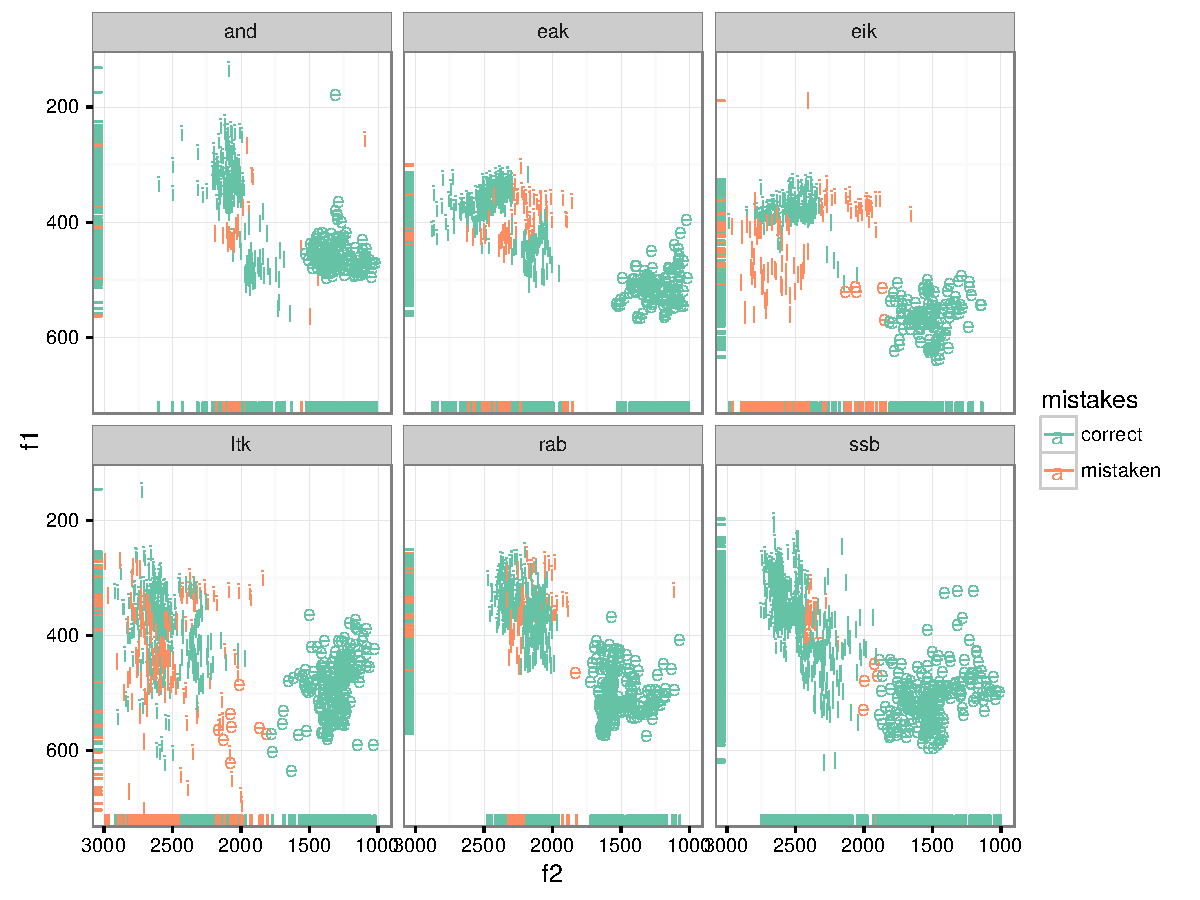
\includegraphics[width=\linewidth]{nanaikmeansmistakes.pdf}
\end{frame}
\subsection{hierarchical}
\begin{frame}{Иерархическая кластеризация}
Иерархические кластеризации имеют два типа:
\begin{itemize}
\mytem \textbf{снизу вверх (agglomerative)}: каждое наблюдение в начальной позиции является кластером, дальше два ближних кластера соединяются в один, а дендограмма отображает порядки таких соединений.
\mytem \textbf{сверху вниз (divisive)}: все наблюдения в начальной позиции являются кластером, который дальше делится на более мелкие, а дендограмма отображает порядки таких разъединений.
\end{itemize}
Алгоритмы иерархической кластеризации требуют на вход матрицы расстояний. Алгоритмов кластерного анализа очень много, так что имеет смысл заглянуть в работу [Gordon 1987] и \alert{\href{http://cran.r-project.org/web/views/Cluster.html}{на страницу CRAN}}.
\end{frame}

\begin{frame}{Иерархическая кластеризация}
Нашим примером снова будет носитель ssb:
\scriptsize
\begin{alltt}
n <- read.csv("http://goo.gl/YPMyl2"{}, sep = ";")\\
n <- n[n\$dictor == "ssb"{},]
\end{alltt}
\normalsize
Функция \scriptsize\verb"hclust"\normalsize\ принимает на вход матрицу расстояний:
\scriptsize
\begin{alltt}
\alert{hc <- hclust(dist(n[,c(5,6)])) \hfill  \# agglomerative clustering\\}
plot(\alert{hc}) \hfill \# график получившихся кластеров\\
plot(\alert{hc}, labels = F) \hfill  \# график без подписей\\
\alert{rect.hclust(\alert{hc}, k=3) \hfill \# выделить k кластеров}
\end{alltt}
\normalsize
Функция \scriptsize\verb"cutree"\normalsize\ возвращает вектор номеров кластеров в соответсвтии с данными, так что можно строить все предыдущие графики:
\scriptsize
\begin{alltt}
cluster <- \alert{cutree(}hc, k=3\alert{)}
\end{alltt}
\normalsize
\begin{center}
\small
\begin{tabular}{lccccccc}
 & and & eak & eik & ltk& rab & ssb \\ 
correct & 393 & 345 & 234 & 478 &494 & 439 \\ 
mistaken & 27 & 142 & 143 & 185 & 157 & 286 \\ 
 &  &  &  &  & & \\ 
 & and & eak & eik & ltk&rab & ssb \\ 
correct & 0.94 & 0.71 & 0.62 & 0.72 & 0.76 & 0.61 \\ 
mistaken & 0.06 & 0.29 & 0.38 & 0.28 & 0.24 & 0.39 \\ 
\end{tabular}
\normalsize
\end{center}
\end{frame}

\begin{frame}{Иерархическая кластеризация}
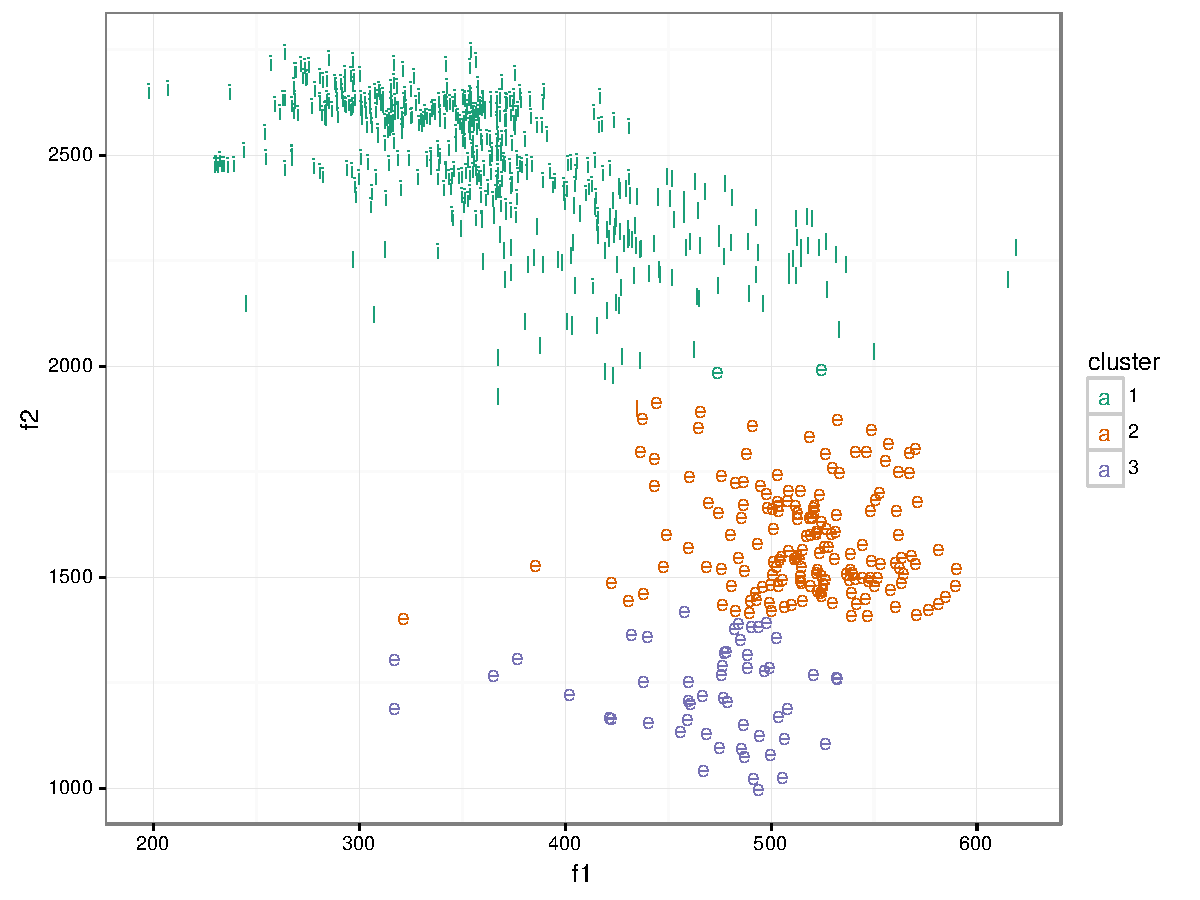
\includegraphics[width=\linewidth]{nanaihc.pdf}
\end{frame}
\begin{frame}{Кластеры иерархическая кластеризации}
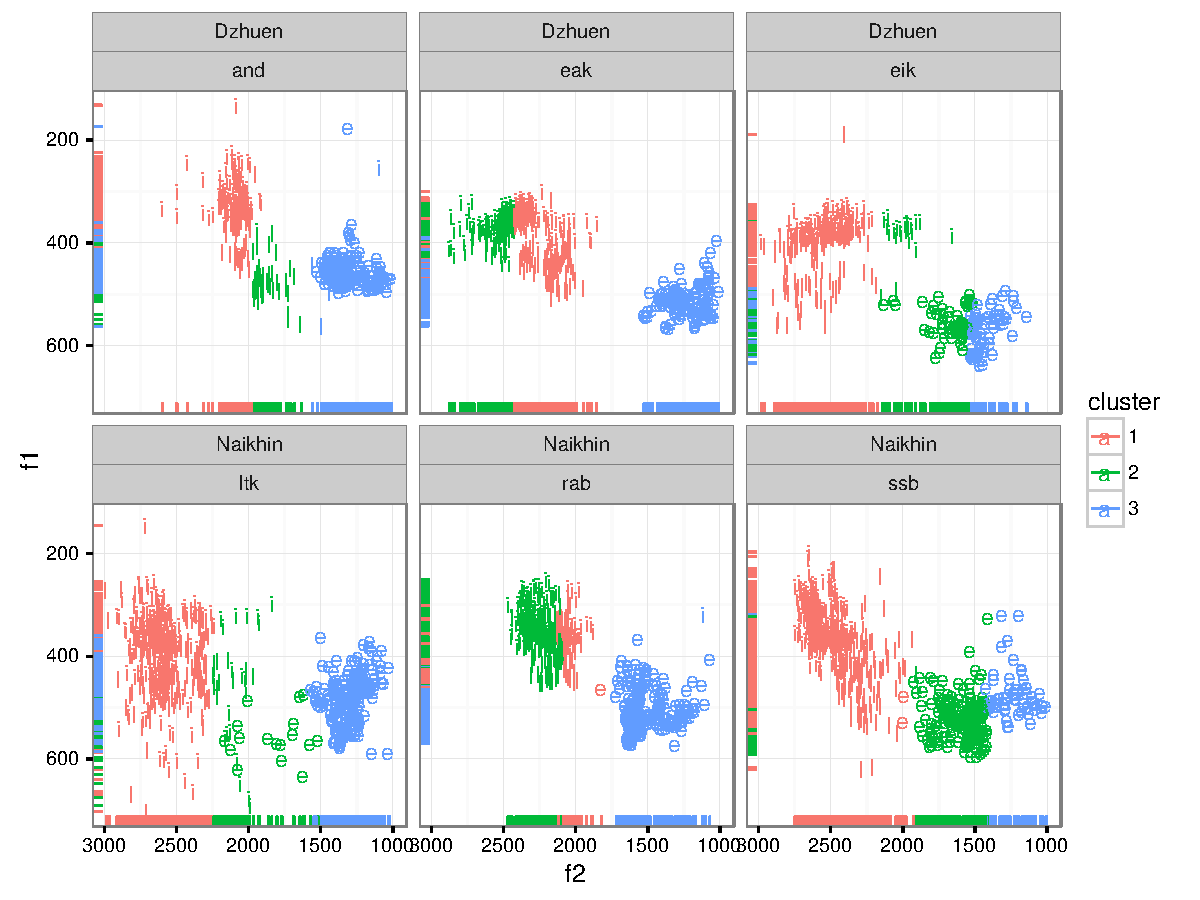
\includegraphics[width=\linewidth]{nanaihcclusters.pdf}
\end{frame}
\begin{frame}{Ошибки алгоритма иерархической кластеризации}
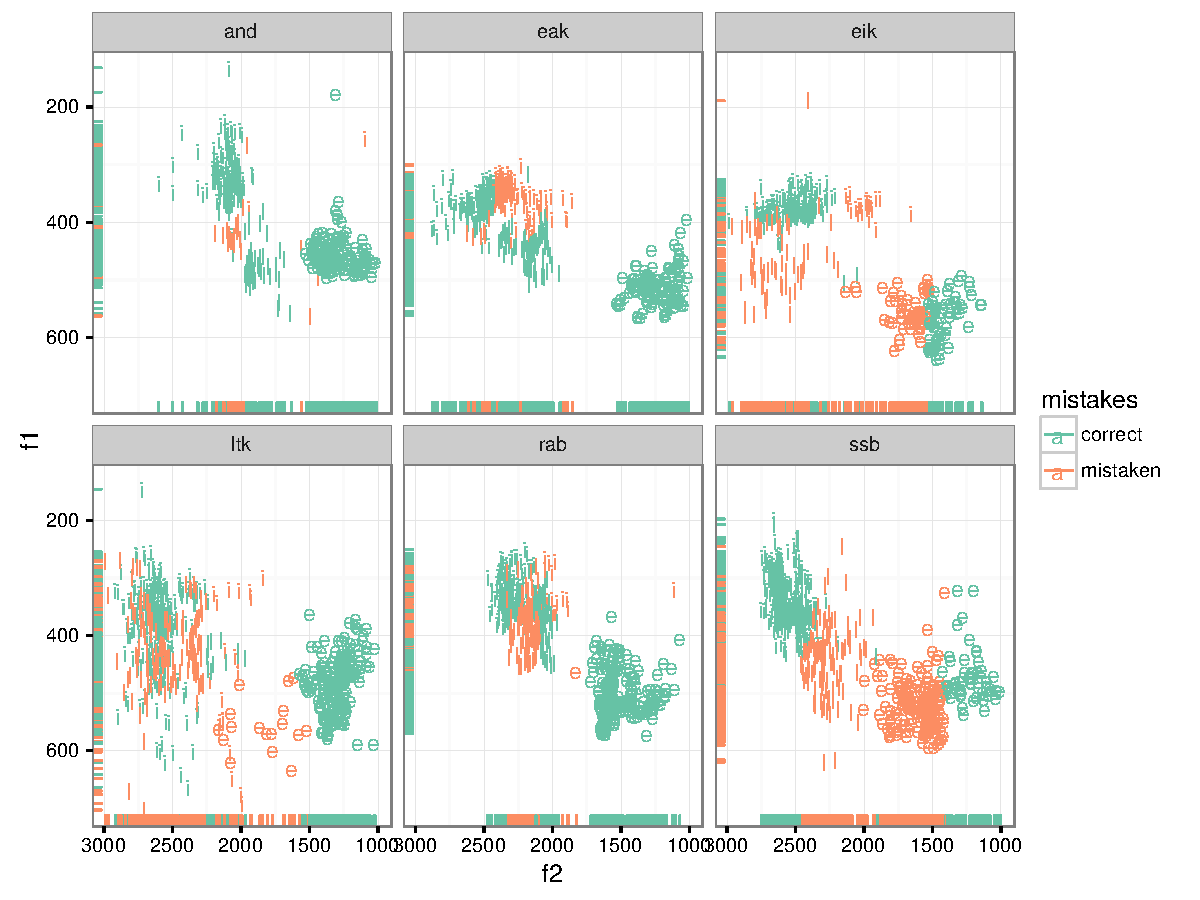
\includegraphics[width=\linewidth]{nanaihcmistakes.pdf}
\end{frame}
\subsection{проблемы}
\begin{frame}{Проблемы приведенных методов}
\begin{itemize}
\mytem $k$-means может давать разные результаты на одних и тех же данных
\mytem при использовании $k$-means нужно знать k
\mytem иерархическая кластеризация не может исправить ошибки, сделанные на предыдущих шагах: в работе \citep{hawkins82} приводится пример вектора  с(-2.2, -2, -1.8, \alert{-0.1, 0.1,} 1.8, 2, 2.2), в котором очевидны три кластера, однако если на первом этапе алгоритм разобьет все на c(-2.2, -2, -1.8, -0.1) и c(0.1, 1.8, 2, 2.2), то дальше это исправлено не будет.
\end{itemize}
\end{frame}
\subsection{дендрограммы}
\begin{frame}{Дендрограммы}
Дендограммой обычно называют граф, отображающий некоторые расстояния между единицами. Существует достаточно много методов построения графов на основе матрицы расстояний, напрямую связанный с используемым методом кластеризации. Надо отметить, что дендограмма это всего лишь \textbf{семейство визуализаций матрицы расстояний}. Примером для построения дендрограмм послужат данные фонетических особенностей адыгских идиомов:\\
\scriptsize
\begin{alltt}
ad <- read.csv("http://goo.gl/Rj92fh")\\
rownames(ad) <- ad[,1]\\
ad.d <- dist(ad, method = "binary")\\
ad.c <- hclust(ad.d)\\
\alert{library(ape)}\\
ad.c <- \alert{as.phylo(}ad.c\alert{)} \hfill \# этот формат лучше воспринимается\\
\alert{plot(ad.c, type = "phylogram")}
\end{alltt}
\normalsize
\end{frame}
\begin{frame}{Дендрограммы: type = "phylogram"}
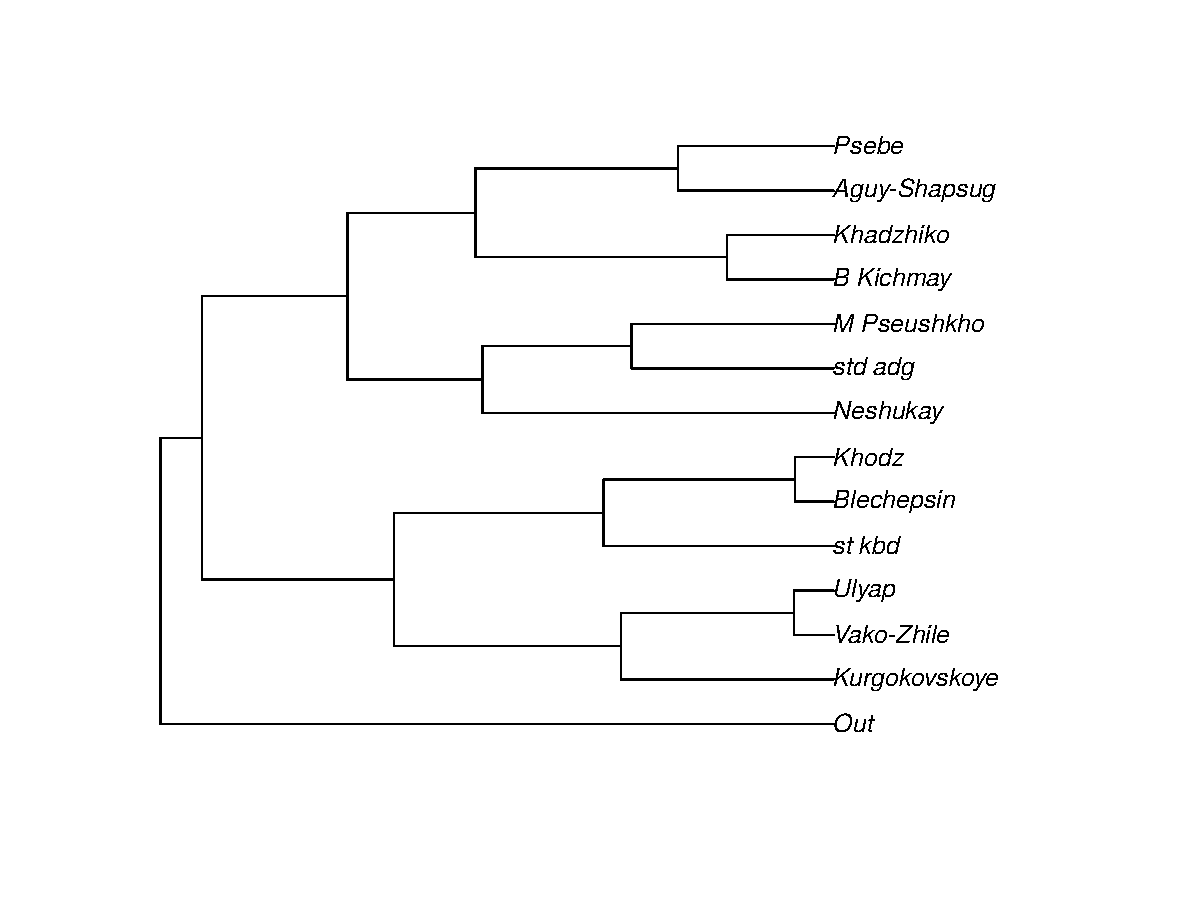
\includegraphics[width=\linewidth]{dendrrect.pdf}
\end{frame}
\begin{frame}{Дендрограммы: type = "cladogram"}
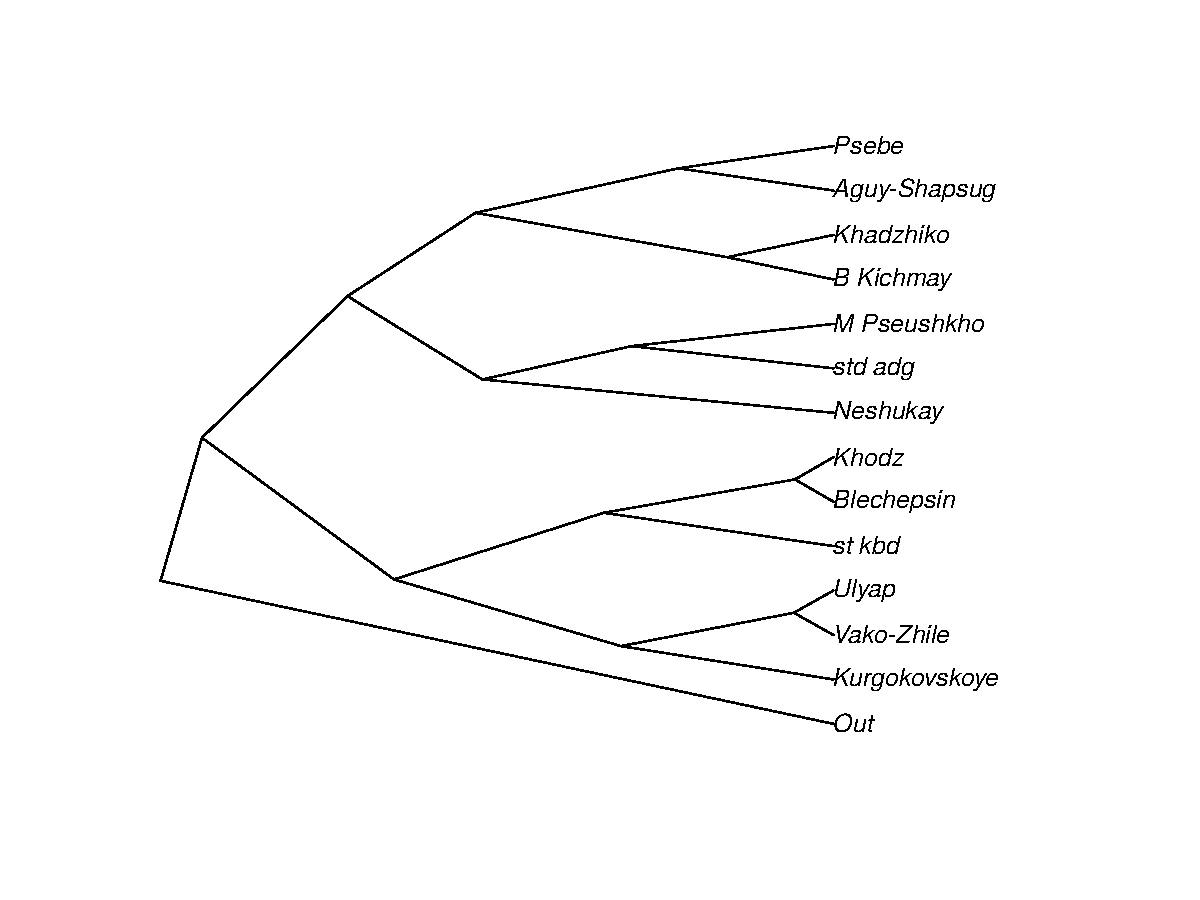
\includegraphics[width=\linewidth]{dendrclad.pdf}
\end{frame}
\begin{frame}{Дендрограммы: type = "unrooted"}
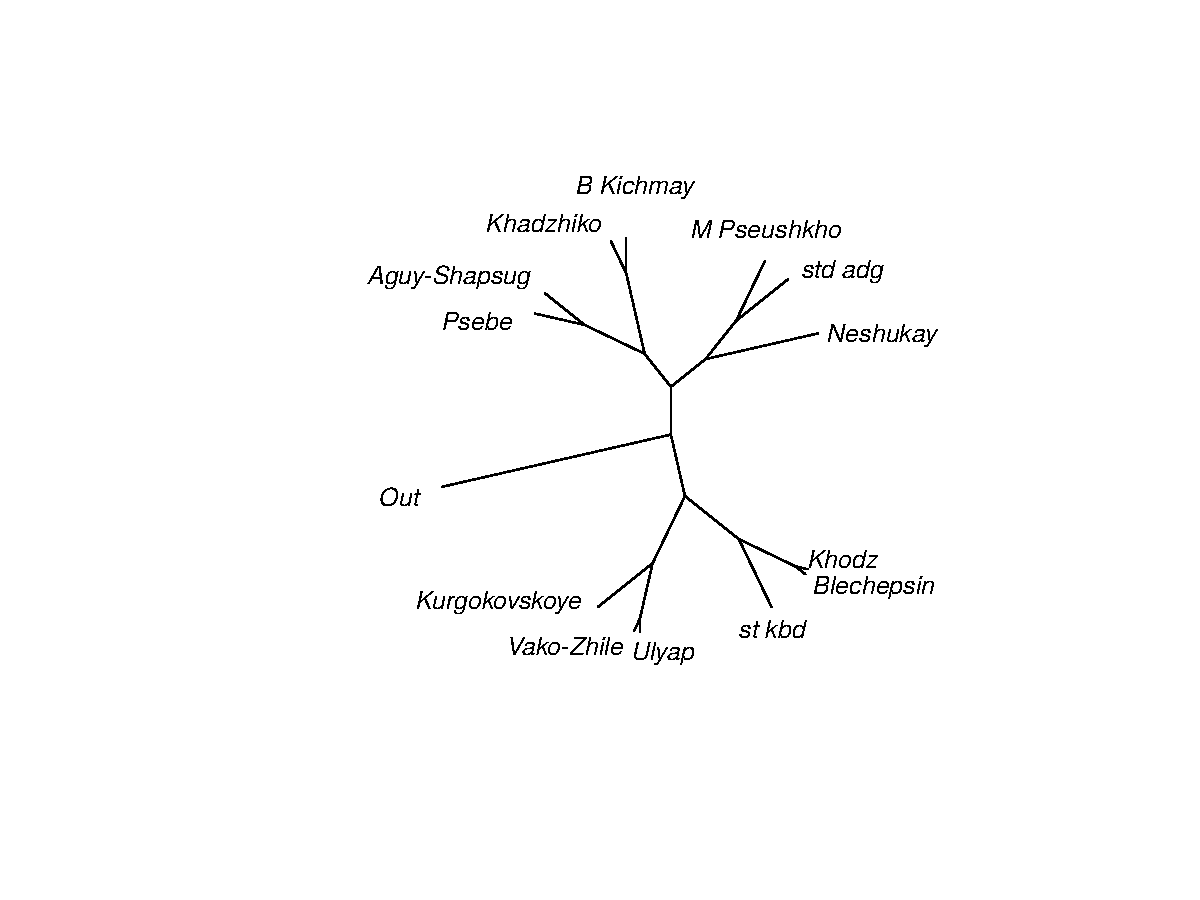
\includegraphics[width=0.7\linewidth]{dendu.pdf}\\
Плохо работает, нужно доводить руками.
\end{frame}
\begin{frame}{Дендрограммы: type = "fan"}
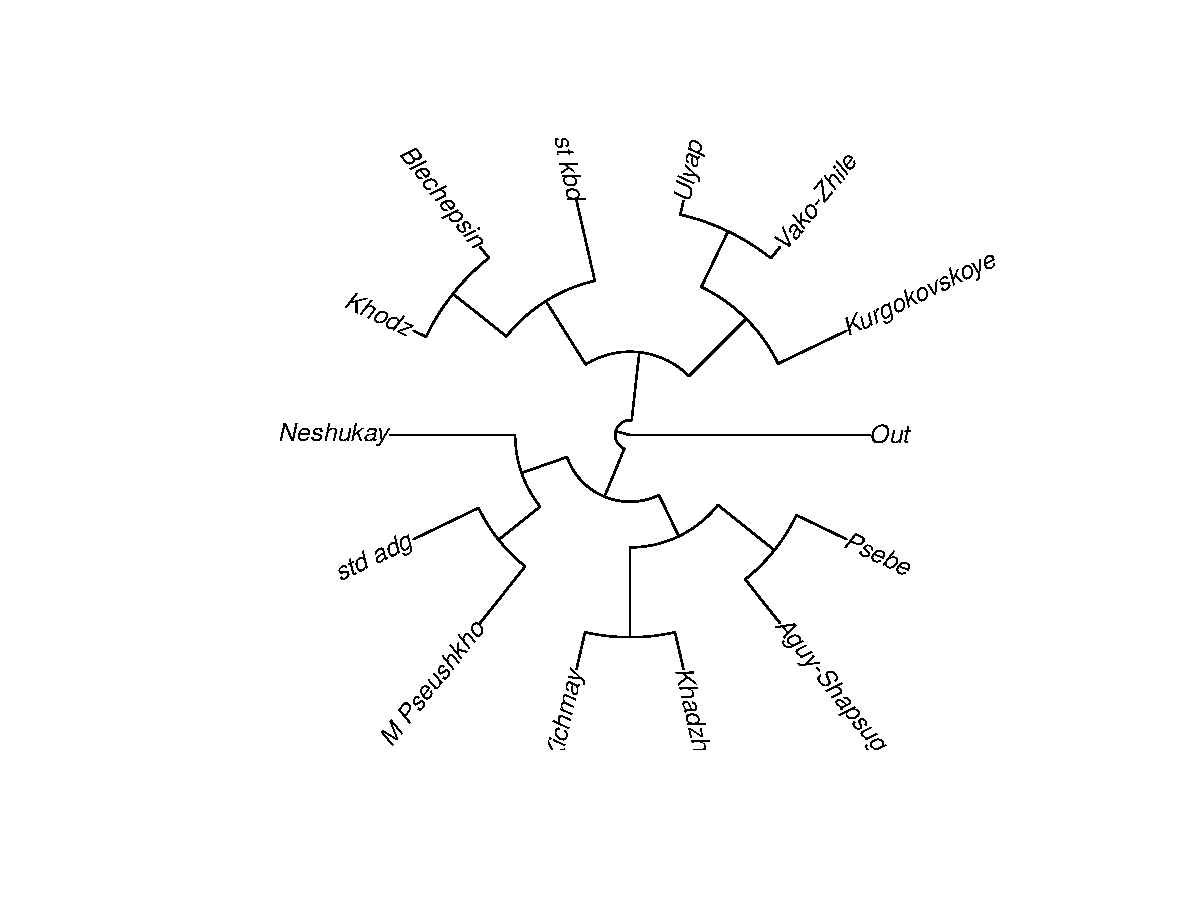
\includegraphics[width=\linewidth]{dendfan.pdf}
\end{frame}
\begin{frame}{Дендрограммы: type = "radial"}
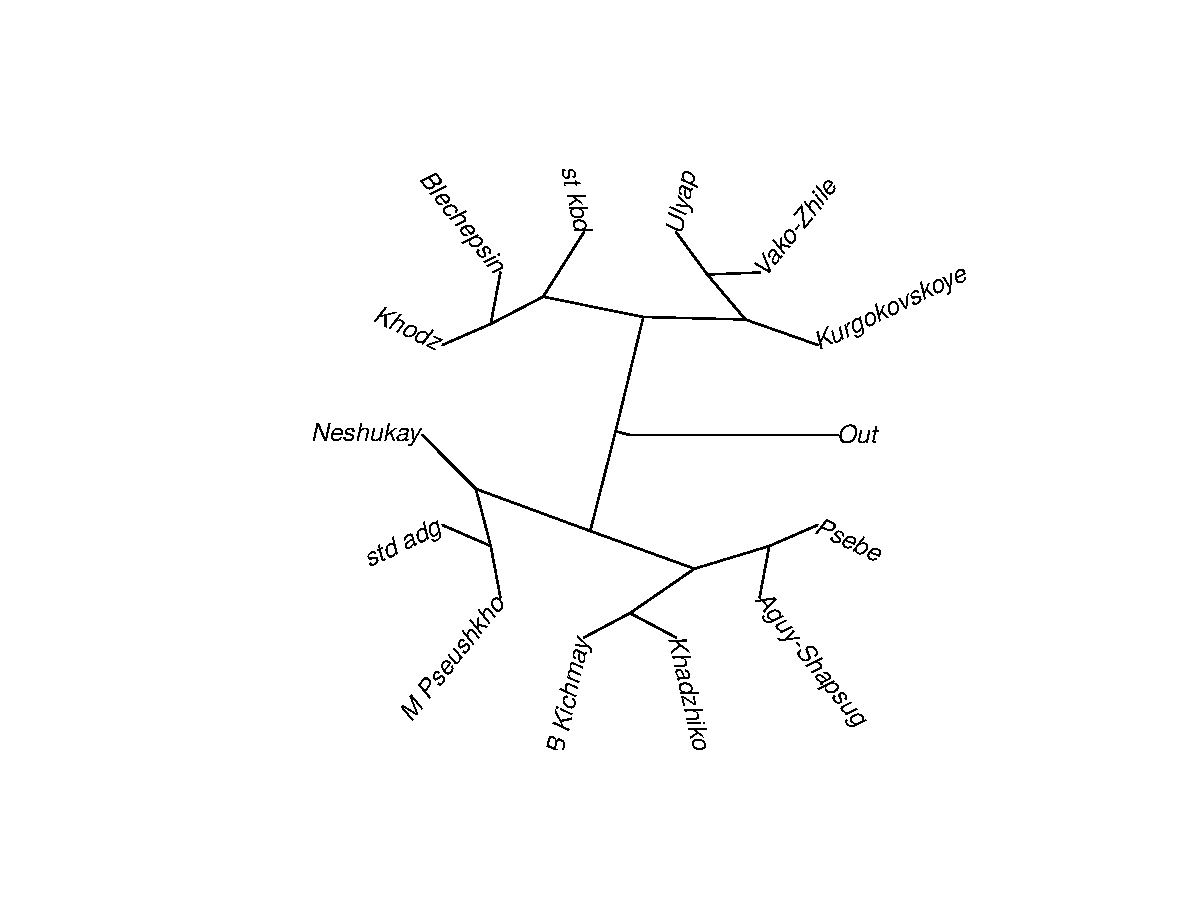
\includegraphics[width=\linewidth]{dendradial.pdf}
\end{frame}
\subsection{валидация кластеров}
\section{деревья решений}
\begin{frame}{Деревья решений}
Достаточно популярным средством построения моделей является дерево решений. В узлах дерева пишутся условия, ограничивающие предикторы, на ребрах записываются значения предикторов, а на листьях дерева записаны значения предсказываемой переменной. Деревья решений позволяют решать как задачи регрессии, так и классификации.
\vspace{-3mm}
\begin{multicols}{2}
\begin{itemize}
\item[pro]  ДР легко интерпретировать
\item[pro] ДР могут работать с переменными любого типа
\item[pro] ДР автоматически подбирают модель, учетывая взаимодействия
\columnbreak
\item[contra] Даже незначительные изменения в обучающих данных могут привести к значительной перестройке модели
\item[contra] Невысокая предсказательная точность
\end{itemize}
\end{multicols}
Для преодоления недостатков можно использовать \textbf{случайные леса (random forest)} и другие ансамбли деревьев.
\end{frame}
\begin{frame}{Деревья решений}
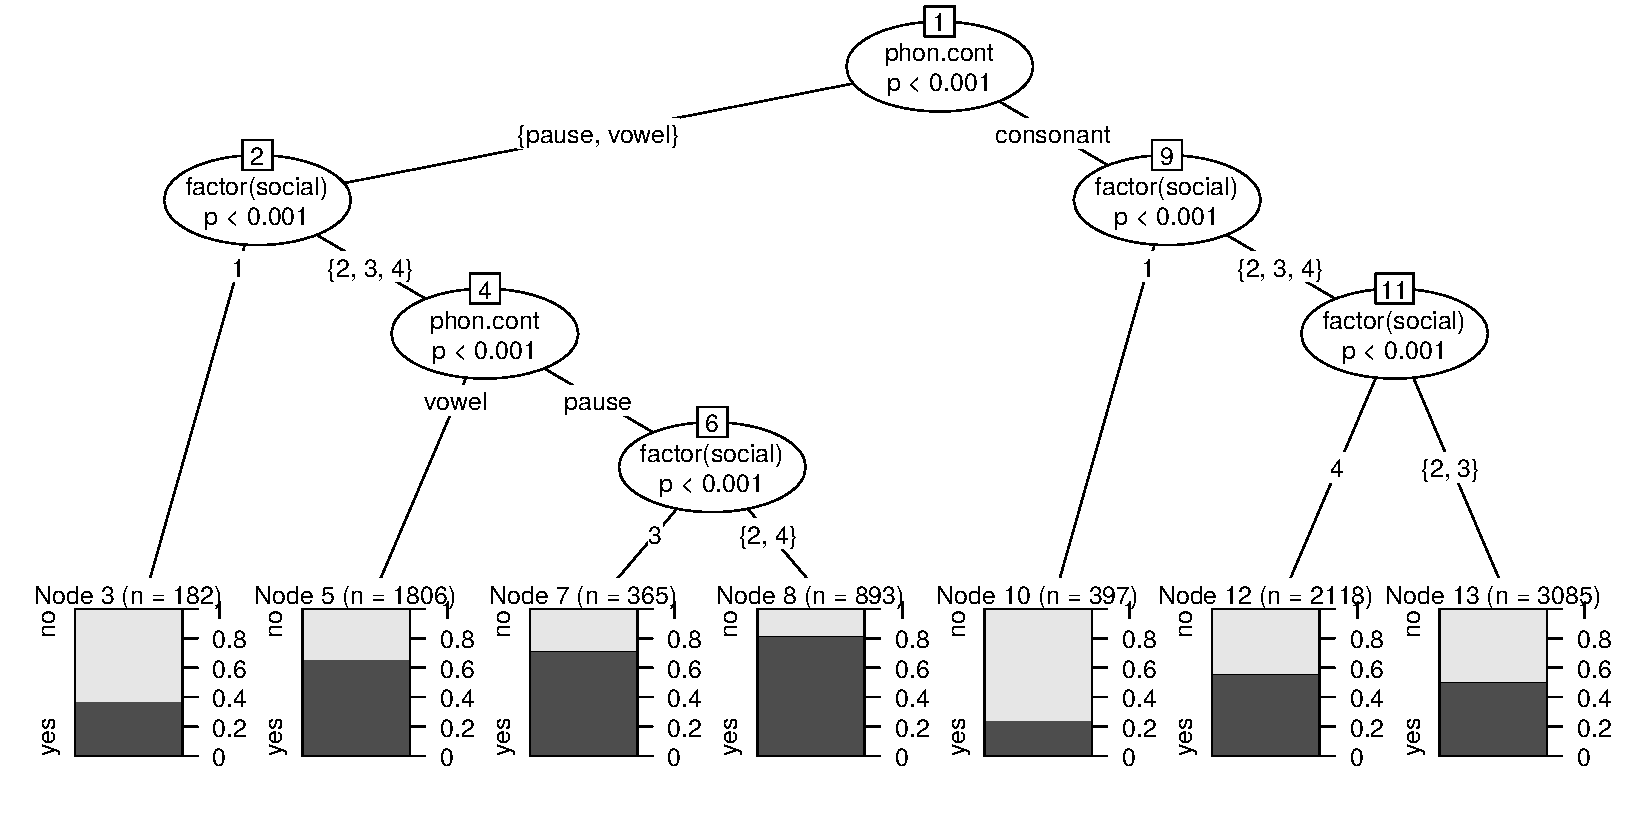
\includegraphics[width=\linewidth]{dtree}\\
\scriptsize
\begin{alltt}
df <- read.csv("http://goo.gl/NwbKsN") \\
df\$social <- \alert{factor(df\$social) \hfill \# внимание! числовой vs. номинативный}\medskip\\
\alert{library(party)} \\
fit <- \alert{ctree(}deletion\textasciitilde phon.cont+social, data=df\alert{)}\\
plot(fit)
\end{alltt}
\normalsize
\end{frame}
\begin{frame}
{\huge Спасибо за внимание\bigskip\\
\normalsize Пишите письма\\
agricolamz@gmail.com
\vspace{-130pt}}
\end{frame}
\begin{frame}{Список литературы}
\footnotesize
\bibliographystyle{chicago}
\bibliography{bibliography}
\end{frame}
\end{document}